\chapter{Introducci\'on}
\label{cap:intro}

\section{Antecedentes y motivaci\'on}
\label{intro:motivacion}

Un grupo de científicos del Departamento de Física de la Universidad de Santiago de Chile trabaja en la simulación de los efectos del campo magnético en los átomos de distintos objetos, tomando en cuenta su forma, su material y su distribución atómica, entre otras características, usando una aplicación escrita en C empleando el Método de Monte Carlo \citep{MonteCarlo}.

No obstante lo anterior, uno de los grandes problemas de los científicos es que el proceso previo y posterior a la simulación es ``manual'', para definir el objeto deben hacer un dibujo en Microsoft Paint\textregistered, el cual es analizado por un \emph{script} de Matlab\textregistered\ que debe ser modificado para reflejar las características del objeto en específico que se quiere simular. Para generar imágenes para, por ejemplo, una publicación, también deben ejecutar ciertos \emph{scripts}, sin embargo esto es aún más complicado, ya que deben hacer ensayo y error hasta conseguir que la imagen sea representativa del resultado, puesto que muchas veces tienen errores de visualización que no reflejan el estado real. Estos dos sub-procesos hacen que el proceso de simulación sea tedioso, quitando mucho tiempo que podría ser usado en analizar los resultados.

Es aquí donde la informática puede contribuir, creando aplicaciones que mejoren estos procesos, que valoricen el tiempo de los científicos. Por consiguiente esta es una oportunidad única de ayudar a la obtención de conocimientos que permitan entender el entorno y de mejorar los procesos que permiten avanzar como sociedad hacia la comprensión del universo.


\section{Descripci\'on del problema}
\label{intro:problema}

Actualmente no existe un método estándar de diseño de objetos para aplicar la simulación Monte Carlo, que permita definir características físicas y geométricas y crear un archivo de entrada, que describa cada uno de los átomos, para la simulación, por lo que cada nuevo investigador en general usa como base las herramientas generadas por antiguos tesistas y lo van modificando para aplicarlo a sus investigaciones. Tampoco existe una solución para la visualización de los resultados entregados y la posterior exportación de estos para publicaciones y conferencias.

\section{Proceso actual}

\subsection{Diseño de objetos para simular}

Actualmente los científicos no tienen un proceso definido y formal de creación de objetos sobre los cuales se van a simular, ya que existen diversas soluciones implementadas a través del tiempo, desde \emph{scripts} que fueron creados especialmente para diseñar un objeto en específico hasta uno más flexible, pero igualmente engorroso, usando como base un mapa de bits.


\subsubsection{Diseño programático de objetos}

La primera opción para diseñar objetos sobre los cuales se correra la simulación es de manera programática, es decir, escribiendo un \emph{script} que defina todas las partículas de un objeto y sus vecindades, para alguien con experiencia en esta área puede ser relativamente sencillo diseñar algunos objetos regulares, como por ejemplo un cilindro, no obstante esto se complica si se quieren diseñar estructuras irregulares. Dado que la visualización del objeto diseñado es de muy baja calidad con este sistema es fácil cometer errores que eventualmente pueden invalidar los resultados de una simulación.

\begin{figure}[H]
  \centering
  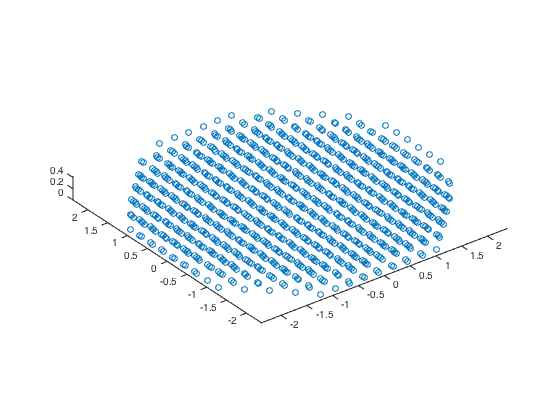
\includegraphics[scale=.6]{images/procesoActualScript}
  \caption{\em Ejemplo de imagen salida de un \emph{script} de generación de objeto}
\end{figure}

\subsubsection{Diseño en base a mapa de bits}
\label{intro:procesoactualmapa}

\noindent
\begin{figure}[H]
  \centering
  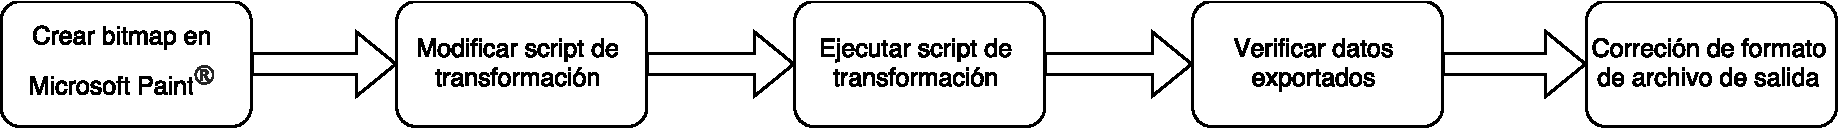
\includegraphics[scale=.5]{images/procesoActualBitmapFlujo}
  \caption{\em Flujo para creación de diseño en base a mapa de bits}
\end{figure}

Para flexibilizar el diseño de objetos y bajar la posibilidad de errores se creó un sistema que permite hacer este proceso basándose en un mapa de bits, de tal forma que ya no fuese necesario programar todo desde cero, si no que bastaba con crear una imagen que representara la primera capa del objeto y usar el script correcto en base a los parámetro físicos de este.

Para iniciar este proceso es necesario tener un editor de imágenes que permita crear archivos .bmp, como por ejemplo Microsoft Paint\textsuperscript{\textregistered}, luego crear una imagen del tamaño deseado, la cual usualmente no excede los 50px x 50px, y ampliarla al máximo de forma de poder trabajar a nivel de pixeles. Luego se deben pintar, con color negro, los pixeles que representen la primera capa de átomos del objeto, estos pixeles luego serán identificados por un \emph{script} de \emph{Matlab}.

En la siguiente imagen se muestra un ejemplo de estos mapas, usando una imagen de 10px x 10px, con una cruz centrada.

\begin{figure}[H]
  \centering
  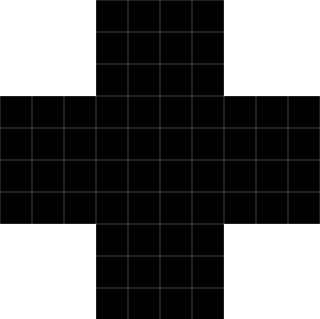
\includegraphics[scale=.6]{images/procesoActualBitmap}
  \caption{\em Mapa de bits de 10px x 10px}
\end{figure}

Luego deben modificar un \emph{script} de \emph{Matlab}, el cual tiene múltiples versiones según el tipo de estructura cristalina que se quiera diseñar, de tal forma de ingresar los parámetros físicos del objeto. Algunas de las opciones que se deben configurar antes de iniciar la ejecución son:

\begin{description}
	\item [Número de capas] \hfill \\
		Cuantas veces se repite la primera capa para formar un objeto en 3D.
	\item [Coeficiente de escalamiento] \hfill \\
		Es un coeficiente usado para dar al objeto las medidas deseadas para ejecutar la simulación.
	\item [Constante de red] \hfill \\
		Esta es la dimensión de la arista de una celda unitaria
\end{description}

Todos estos parámetros deben ser modificados directamente en el código, en distintas partes de este, por lo que es muy fácil cometer errores, los que por supuesto invalidan cualquier simulación hecha en base a estos.

Una vez configurado el script debe ser ejecutado, este leerá el mapa de bits ingresado como parámetro analizando cada uno de los pixeles, creando un arreglo binario de 2 dimensiones, donde un pixel negro es representado por 1 y un pixel blanco es representado por un 0, lo que creará la primera capa de partículas; luego, según las configuraciones ingresadas, generará el resto de partículas buscadas y sus vecindades, provocando como salida un archivo con las posiciones de los átomos y sus vecinos, además de dos imágenes que representan las distintas partículas generadas en base a los archivos de entrada, estas imágenes no son lo suficientemente claras como para poder identificar errores en el diseño esperado, por lo que la posibilidad de equivocarse y simular con una premisa inválida es algo mucho más común que lo esperado.

\begin{figure}[H]
  \centering
  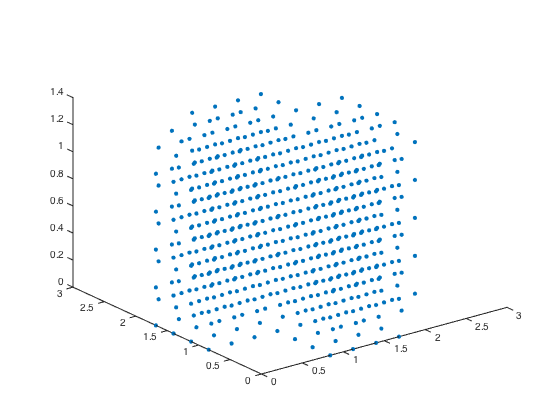
\includegraphics[scale=.6]{images/procesoActualMatlab1}
  \caption{\em Vista 3D de los átomos encontrados}
\end{figure}

\begin{figure}[H]
  \centering
  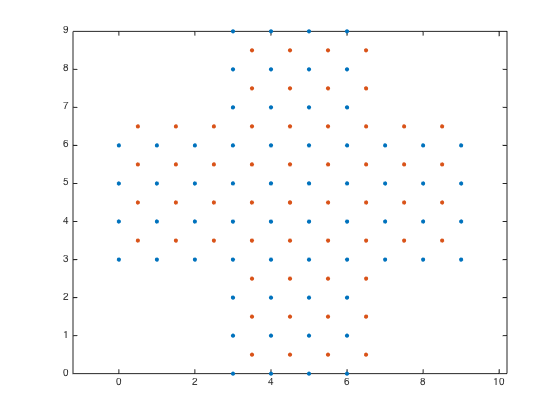
\includegraphics[scale=.6]{images/procesoActualMatlab2}
  \caption{\em Vista 2D de la primera capa de átomos}
\end{figure}

Una vez decidido que el objeto diseñado se usará para una simulación es necesario ejecutar un nuevo software, escrito en C, que se encargará de modificar el archivo de salida del script de \emph{Matlab} de tal forma de que pueda ser usado como entrada para la simulación Monte Carlo. Cabe notar que este software está compilado y no se cuentan con el código de fuente de este, de tal forma que si en algún momento se necesitara modificar el formato de la entrada de la simulación este software se debería re-escribir.

\begin{center}
	\begin{lstlisting}
		5.4700000e+02   1.4000000e-01   1.5400000e+00   1.2600000e+00   4.0000000e+00   4.8300000e+02   4.8400000e+02   4.8700000e+02   4.8800000e+02   0.0000000e+00   0.0000000e+00   0.0000000e+00   0.0000000e+00
	\end{lstlisting}
	\em Formato de salida generado por el script de matlab
\end{center}

\begin{center}
	\begin{lstlisting}
		547   0.14   1.54   1.26   4   483   484   487   488   0   0   0   0
	\end{lstlisting}
	\em Formato de entrada necesario para la simulación
\end{center}

Además de modificar el formato de todas las líneas del archivo generado este software agrega una línea en el inicio del archivo que contiene distintos parámetros usados por el software de simulación, como el número de partículas y la constante de escalamiento.

\subsection{Visualización de resultados}

Si bien el proceso de diseño de objetos es precario este no se compara con el de visualización y exportación de resultados, tanto en forma de imágenes como videos. Dentro de las limitaciones que tienen es la imposibilidad de generar videos con colores que permitan distinguir una tercera dimensión no clara al ser una representación en 2D.

Actualmente se usa la funcionalidad \emph{Quiver plot} de matlab, que permite dibujar rápidamente vectores en base a archivos de entrada con cierto formato, no obstante este proceso requiere de tiempo para obtener representaciones que realmente reflejen lo deseado, siendo un proceso de ensayo y error que gasta tiempo de manera innecesaria para los científicos.


% Actualmente los investigadores deben preparar la simulación usando un \emph{script} en Matlab\textregistered, el cual analiza un archivo \emph{.bmp} creado en \emph{Microsoft Paint\textregistered}, esta imagen generalmente es pequeña, menor a 50px x 50px, y representa la primera capa del objeto (mirado desde arriba), para esto se marcan los pixeles que describen el objeto, de esta forma el mapa de \emph{bits} es binario, si un \emph{pixel} es negro se considera un 1, si es blanco se considera un 0. En este \emph{script} se describen características específicas del objeto que se quiere definir, entre ellos:
% \begin{itemize}
% 	\item Número de capas: Cuantas veces se repite la primera capa para formar un objeto en 3D.
% 	\item Distribución de los átomos (ver anexo A): Como premisa se trabaja sólo con distribuciones cúbicas de átomos, no obstante estas distribuciones tienen ciertas características específicas, por ejemplo:
% 	\begin{itemize}
% 		\item Cúbico simple (SC por \emph{Simple Cubic}): En cada vértice de una distribución cúbica se encuentra un átomo.
% 		\item Centrado en las caras (FCC por \emph{Face-centered Cubic}): Además del átomo en cada vértice de la distribución cúbica, hay un átomo en el centro de cada cara de la distribución.
% 		\item Centrado (BCC por \emph{Body-centered Cubic}):  Además del átomo en cada vértice de la distribución cúbica, hay un átomo en el centro de cada distribución.
% 	\end{itemize}
% 	\item Coeficiente de escalamiento: Es un coeficiente usado para dar al objeto las medidas deseadas para ejecutar la simulación.
% \end{itemize}

% Este proceso produce un archivo de texto plano describiendo cada uno de los átomos del objeto sobre el cuál se aplicará la simulación.

% Luego de ejecutada la simulación el software entrega múltiples archivos de texto, uno que define cada uno de los átomos con un ID y una posición en el espacio, y N archivos que definen la fuerza magnética de cada átomo en un tiempo dado. Los científicos deben seleccionar uno de estos archivos y aplicar un \emph{script} de Matlab\textregistered\ para poder visualizar el resultado.

% El proceso de exportación de imágenes para publicaciones puede tomar un día de trabajo para los científicos, ya que deben hacer ``ensayo y error'' hasta que la imagen producida refleje lo que desean. Luego deben esperar por la aprobación por parte del profesor guía, en caso de ser rechazada, deben volver a ejecutar el proceso.

% \subsection{Soluciones similares}
% Existe una herramienta que hace simulaciones similares a las que hace el grupo de científicos llamada ``Go Parallel Magnet\textregistered''. A pesar de que la simulación no es exactamente la misma, el flujo de diseño es útil para el proyecto. Sin ir más lejos los científicos basan el proceso actual en éste.

% ``Go Parallel Magnet\textregistered'' usa para el diseño un sistema de multi-capas, donde se define la capa superior del objeto y se indica la cantidad de veces que ésta se repetirá. Con estos datos se crea un objeto en 3D que luego se transforma en la estructura molecular deseada.

\section{Propósitos de la solución}
\begin{enumerate}
  \item Mejorar el proceso de preparación de la simulación.
  \item Mejorar el proceso de exportación de imágenes para publicaciones.
\end{enumerate}


\section{Alcances o limitaciones de la solución}
\begin{itemize}
	\item El software se encargará del diseño de objetos para la simulación entregando la entrada para ésta y posteriormente de la visualización de los resultados, y de la exportación de estos para publicaciones, mas \textbf{NO} se encargará de la simulación en sí y queda fuera del alcance de la solución.
	\item La aplicación estará disponible para sistema operativo MAC OS X.
	\item El diseño de objeto será por capas, es decir, se define la ``vista superior'' y la cantidad de veces que se repetirá hacia abajo.
\end{itemize}

\section{Objetivos y alcance del proyecto}
\label{intro:objetivos}

\subsection{Objetivo general}
Crear un software que permita diseñar objetos en 3D, con características físicas y geométricas específicas, sobre los cuáles se aplicarán simulaciones de campo magnético a nivel atómico y analizar los resultados de forma visual, permitiendo la exportación de imágenes para publicaciones.

\subsection{Objetivos espec\'ificos}

Para la consecución del objetivo general, se plantean las siguientes metas intermedias para el software:

\begin{enumerate}
  \item Modelar el proceso de simulación del efecto de campo magnético en átomos efectuado por los científicos del Departamento de Física de la Universidad de Santiago de Chile.
  \item Diseñar la herramienta informática de ayuda para la investigación antes mencionada.
  \item Crear el software.
  \item Validar el cumplimiento de los requerimientos.
\end{enumerate}


\section{Características de la solución}

Como solución se propone la creación de un software que facilite el trabajo de los científicos. Esta aplicación se divide en dos funcionalidades:

\subsection{Diseño del objeto sobre el cuál se hará la solución:}

El software debe permitir crear visualmente un objeto en 3D, con ciertas características físicas como la distribución cúbica (ver anexo A). Luego de la creación y configuración del objeto la aplicación debe exportar un archivo de texto que sirva como entrada para el software que hará la simulación. Este archivo tiene un formato ya definido y debe describir la posición de cada átomo del objeto.

Este proceso se divide en tres características:

\begin{enumerate}
	\item Creación de objeto en base a un mapa de \emph{bits} binario, con características pre-definidas, y exportación de archivo de entrada para la simulación.
	\item Permitir la entrada de características del objeto, como número de capas y ordenamiento de los átomos.
	\item Visualización atómica en 3D del objeto sobre el cuál se hará la simulación.
\end{enumerate}

\subsection{Visualización de resultados de la simulación:}

El software debe tomar la totalidad de archivos de salida de la simulación como entrada y debe ser capaz de mostrar visualmente el estado magnético de cada átomo en un tiempo \emph{t}, también debe ser posible ver la simulación animada a través del tiempo, como un video.

La salida de la visualización serán imágenes en 2D del estado de la simulación en un tiempo \emph{t}, estas imágenes deben tener colores que permitan al lector entender el resultado a pesar de la dimensión faltante, por ejemplo, usando la proyección del vector en uno de los ejes y asignando un color según la intensidad de éste.

Este proceso se divide en tres características:

\begin{enumerate}
	\item Permitir ver el estado de la simulación en 3D en un tiempo \emph{t}.
	\item Permitir ver el cambio de estado de la simulación en 3D de forma animada.
	\item Permitir exportar el estado de la simulación en un tiempo \emph{t} en 2D para publicaciones.
\end{enumerate}


\section{Propósitos de la solución}
\begin{enumerate}
  \item Mejorar el proceso de preparación de la simulación.
  \item Mejorar el proceso de exportación de imágenes para publicaciones.
\end{enumerate}


\section{Alcances o limitaciones de la solución}
\begin{itemize}
	\item El software se encargará del diseño de objetos para la simulación entregando la entrada para ésta y posteriormente de la visualización de los resultados, y de la exportación de estos para publicaciones, mas \textbf{NO} se encargará de la simulación en sí y queda fuera del alcance de la solución.
	\item La aplicación estará disponible para sistema operativo MAC OS X.
	\item El diseño de objeto será por capas, es decir, se define la ``vista superior'' y la cantidad de veces que se repetirá hacia abajo.
\end{itemize}


\section{Metodolog\'ia y herramientas utilizadas}
\label{intro:metodologia}

\subsection{Metodolog\'ia}
Dado que se tiene conocimiento de los requerimientos mayores, pero pueden existir detalles al trabajar en un ámbito tan específico como simulaciones físicas, se decidió usar una modificación de Scrum \citep{SCRUM}.

Scrum está pensado para trabajar en equipos con varios desarrolladores, además de los cargos más de gestión, para esto se tienen 3 roles \citep{website:ScrumRoles}:

\begin{description}
  \item[\emph{Product Owner}] \hfill \\
  Es el encargado de maximizar el valor del trabajo el equipo, para esto tiene un alto conocimiento del producto mediante un contacto directo con los \emph{stakeholders} y facilita la comunicación de estos con el equipo de desarrollo, debido a esto es el responsable de decidir qué se va a construir, pero no el cómo. Para este proyecto el \emph{Product Owner} será el profesor Fernando Rannou, quién tiene contacto constante con los \emph{stakeholders} por proyectos paralelos que se están desarrollando.
  \item[\emph{Scrum Master}] \hfill \\
  Es el líder del equipo de desarrollo y debe tener un buen conocimiento de la metodología scrum, el cual debe traspasar al equipo de desarrolladores. Sus 3 principales tareas son: Guíar al equipo teniendo un conocimiento tanto del producto como de las tecnologías a utilizar, mantener al equipo avanzando eliminando toda dificultad que puedan tener durante el desarrollo, estas dificultades pueden ser tanto internas como externas, y enseñar a metodología \emph{scrum} al equipo. En este caso como solo un desarrollador trabajará en el proyecto y este tiene un gran conocimiento de la metodología gracias a sus años de experiencia laboral usandola, no se usará este rol.
  \item[Desarrollador] \hfill \\
  El desarrollador es el encargado de entregar los incrementales del producto, para eso se basa en la lista de tareas definidas por el \emph{Product Owner} al inicio de un \emph{sprint}. En este proyecto solo trabajará un programador.
\end{description}

Otras modificaciones hechas a la metodología fue modificar alguna de sus ceremonias, cambiando la reunión diaria (\emph{Daily Scrum}) por una semanal, entre el profesor y el desarrollador, las reuniones retrospectivas al finalizar cada \emph{sprint} se unió con la de planificación del siguiente periodo de desarrollo. Además, como es recomendado, se tuvo una reunión con los \emph{stakeholders} luego de cada sprint.

Estas modificaciones fueron necesarias para poder usar la metodología en un proyecto con solo un desarrollador y optimizando al máximo el tiempo usado en reuniones, debido al poco espacio en las agendas tanto del desarrollador como del \emph{Product Owner}.

\subsection{Herramientas de desarrollo}
\subsection{Modelado 3D: OpenGL}
Se usará OpenGL como biblioteca de modelado 3D, por ser el estado del arte en este ámbito, entre sus ventajas está el ser multi-plataforma, lo que eventualmente permitiría una rápida portación a otro sistema operativo, y el ser la más usada actualmente, lo que permite que tenga una amplia comunidad de usuarios que la soportan y documentan.

\subsection{Lenguaje de programación: Python}
Para el desarrollo se usará el lenguaje de programación Python con la biblioteca wxPython para Intefaz de Usuario. Esta biblioteca tiene soporte para la API OpenGL. Python, al ser un lenguaje multiplataforma, permitiría una rápida portación a otro sistema operativo en el futuro.

\subsection{Control de versiones: GIT}
Para el versionamiento del código se usará GIT, manteniendo un respaldo del repositorio con el código y la documentación en una máquina virtual con Linux ubicada en Estados Unidos.

\section{Ambiente de desarrollo}
Para el desarrollo se usará el siguiente ambiente de desarrollo:
\begin{itemize}
	\item Computador marca Apple, con una tarjeta gráfica que soporte OpenGL 3.2+ y sistema operativo Mac OS X para el desarrollo.
	\item Una máquina virtual con Linux, ubicada en Estados Unidos, para mantener un respaldo del código y de la documentación.
\end{itemize}
